\documentclass[a4paper,12pt]{article}
\usepackage[utf8]{inputenc}
\usepackage{listings}
\usepackage[table]{xcolor}
\usepackage{graphicx}

\graphicspath{{/Users/tom/Documents/Programmieren/ChemBox/Documentation/Images/}}

\usepackage{algpseudocode}
\usepackage{algorithm}

% Redefine the keywords to use the new command
\algrenewcommand\algorithmicif{\textbf{IF}}
\algrenewcommand\algorithmicthen{\textbf{THEN}}
\algrenewcommand\algorithmicelse{\textbf{ELSE}}
\algrenewcommand\algorithmicend{\textbf{END}}
\algrenewcommand\algorithmicfor{\textbf{FOR}}
\algrenewcommand\algorithmicdo{\textbf{DO}}
\algrenewcommand\algorithmicwhile{\textbf{WHILE}}
\algrenewcommand\algorithmicloop{\textbf{LOOP}}
\algrenewcommand\algorithmicrepeat{\textbf{REPEAT}}
\algrenewcommand\algorithmicuntil{\textbf{UNTIL}}
\algrenewcommand\algorithmicreturn{\textbf{RETURN}}
\algrenewcommand\algorithmicfunction{\textbf{SUBROUTINE}}



\usepackage{tikz}
\usetikzlibrary{shapes.geometric, arrows}

\tikzstyle{startstop} = [rectangle, rounded corners, minimum width=3cm, minimum height=1cm,text centered, draw=black, fill=red!30]
\tikzstyle{io} = [trapezium, trapezium left angle=70, trapezium right angle=110, minimum width=3cm, minimum height=1cm, text centered, draw=black, fill=blue!30]
\tikzstyle{process} = [rectangle, minimum width=3cm, minimum height=1cm, text centered, draw=black, fill=orange!30]
\tikzstyle{decision} = [diamond, minimum width=3cm, minimum height=1cm, text centered, draw=black, fill=green!30]
\tikzstyle{arrow} = [thick,->,>=stealth]

\definecolor{codegreen}{rgb}{0,0.6,0}
\definecolor{codegray}{rgb}{0.5,0.5,0.5}
\definecolor{codepurple}{rgb}{0.58,0,0.82}
\definecolor{backcolour}{rgb}{0.95,0.95,0.92}

\lstdefinestyle{mystyle}{
    backgroundcolor=\color{backcolour},   
    commentstyle=\color{codegreen},
    keywordstyle=\color{magenta},
    numberstyle=\tiny\color{codegray},
    stringstyle=\color{codepurple},
    basicstyle=\fontsize{8}{10}\ttfamily,
    breakatwhitespace=false,         
    breaklines=true,                 
    captionpos=b,                    
    keepspaces=true,                 
    numbers=left,                    
    numbersep=5pt,                  
    showspaces=false,                
    showstringspaces=false,
    showtabs=false,                  
    tabsize=2,
}

\lstset{style=mystyle}


\title{ChemBox Project Documentation}
\author{Tom Schneider}

\begin{document}
\begin{titlepage}
    \begin{center}
        \vspace*{1cm}
        
        \huge ChemBox Project Documentation
        
        \vspace{1cm}
        
        \Large Tom Schneider
        
        \vfill
        
        \textbf{Date:} \today \\
        
        \vspace{1cm}
        
        \textbf{Center Number:} 29065 \\
        \textbf{Candidate Number:} 7638 \\
        
        \vspace{1cm}
        
        \textbf{Ellesmere College}
        
    \end{center}
\end{titlepage}

\tableofcontents

\pagebreak

\section{Analysis}

\subsection{Introduction}

Technology gives us the benefits of saving time and doing work more efficiently. The use of software and technology in chemistry does not only help increase accuracy and decrease human error, but also reduces the time spent performing repetitive tasks by hand. ChemBox is a software project with the aim of creating an interactive, user-friendly and intuitive toolbox for automating and simplifying complex and repetitive tasks that come up on a daily basis for students, educators and professionals in the field of chemistry. The application features a range of different tools that should help chemists work more efficiently and also carry out their work more accurately. ChemBox is split into three distinct modules with different functionalities.\\
\linebreak
The first module is the "ChemCalculator". The aim of this part of the program is to help the user carry out calculations by filling in equations and formulae. Although substituting numbers into predefined equations is a rather trivial task, it leaves a lot of room for human error when it comes to things like converting between units or applying mathematical laws correctly. This module should help the user with the most important and at the same time most trivial tasks in chemistry.\\
\linebreak
The second module, "ChemBalancer", is for balancing chemical equations, as the name already suggests. Chemical equations come up in every lab experiment, calculation or research problem. While balancing short equations made up of very few different elements is arguably a rather easy task, it can get quite tricky when you have to work with a large number of different elements, complex ions or just very long equations. Making just a tiny mistake when balancing an important equation can cause a big set back as it can take long to find small errors like mixing up a 2 with a 3.\\
\linebreak
The third and last module is the "ChemEditor". Visualising molecular structures can play a vital role in understanding a substances chemical properties or understanding interactions with other substances. Drawing molecules out by hand is pretty straight forward. It is knowing when a bond is valid and which atoms bond together and which don't that is the tricky part. Having a tool that can help you make sure the chemical molecule you want to draw can even exist, can be a great help not only for beginner level chemists but also for more experienced chemists.

\newpage

\subsection{Prospective Users}

Chembox will provide valuable tools to a diverse user base, spanning from students to professional chemists. The intuitive and straight forward design will allow users with varying backgrounds and degrees to use ChemBox for their own specific needs.\\
In the early stage, the main users of this system will be pupils and staff attending Ellesmere College, but it could be a goal to make the software available open source to anyone online.\\
Engaging with pupils at the college during the early stages allows for a valuable user feedback loop. This direct interaction with the user group will provide insights into the software's usability, identify potential improvements, and address any specific requirements that may arise within the college context.


\subsection{Specific Objectives}

Through being an A-Level Chemistry student myself, I have learned a lot about using chemical equations and performing calculations as well as balancing chemical equations and visualising chemical substances and molecules. I was able to identify a number calculations that processes that come up on a regular basis and divide them into non-negotiable and nice-to-have objectives.

\subsubsection{Chemical Equations and Calculations - ChemCalculator}

The first module of the program is for performing  calculations which are based on chemical formulae.
Where appropriate the program should allow the user to choose from a range of different units for each calculation, so the user doesn't have to calculate the conversions like the one from $cm^{3}$ to $dm^{3}$ for example.\\
\linebreak
Required functionalities:\\
\linebreak

\begin{enumerate}

\item Standard moles calculation:
\[moles=\frac{mass}{molar\: mass}\]
\item Calculation to find the concentration:
\[concentration=\frac{moles}{volume}\]
\newpage
\item Avogadro's number calculations. The user should be able to give a number of different inputs, including mass, moles, molecular weight and the number of atoms. After giving two independent inputs, the program should be able to calculate the rest of the values using Avogadro's number.\\
The equation the calculator will be based on is:
\[number\: of\: atoms = Avogadro's\: number \times moles\]
This should be paired with a mole calculator for the possibility use the following formula:
\[number\: of\: atoms = Avogadro's\: number \times \frac{mass}{molar\: mass}\]
\item Atom Economy calculation:
\[Atom\: Economy = \frac{Mr\: of\: desired\: product}{Sum\: of\: Mr\: of\: all\: reactants}\times 100\]
\item Percentage Yield calculation:
\[\%Yield = \frac{Actual\: yield}{Theoretical\: yield} \times 100\]
\item Calculation for the Specific Heat Capacity and Enthalpy changes:
\[q = mc {\Delta} T\]
\begin{quote}
(q = energy change) (m = mass) (c = specific heat capacity) (${\Delta}$T = temperature change)
\end{quote}
\item Equilibrium Constant calculation for a reversible reaction:
\[a[A] + b[B] \rightleftharpoons c[C] + d[D]\]
\[K_{C} = \frac{[C]^{c}[D]^{d}}{[A]^{a}[B]^{b}}\]
\begin{quote}
($K_{C}$ = Equilibrium Constant) (Upper case letter = Concentration) (Lower case letter = Moles in Equation)
\end{quote}
\item Rate Equation and Rate constant calculation:
\[Rate = k[A]^{m}[B]^{n}\]

\end{enumerate}

Non-essential objectives:
\begin{enumerate}
\item Gibbs Free Energy calculation:
\[{\Delta}G = {\Delta}H - T{\Delta}S\]
\begin{quote}
(${\Delta}$G = Gibbs Free Energy) (${\Delta}$H = enthalpy)\\
(T = temperature) (${\Delta}$S = entropy)
\end{quote}
\item Acid calculations - pH and $[H^{+}]$
\[pH = -log[H^{+}]\]
\[[H^{+}] = 10^{-pH}\]
\item Acid dissociation constants $K_{a}$ and $pK_{a}$
\[K_{a} = \frac{[H^{+}][A^{-}]}{[HA]}\]
\[pK_{a} = -logK_{a}\]
\[K_{a} = 10^{-pK_{a}}\]
\end{enumerate}

\newpage

\subsubsection{Chemical Equation Balancer - ChemBalancer}

A substantial part of the project will be the ChemBalancer which will be the module that balances chemical equations. This system must be able to take complex unbalanced equations and convert them into a balanced version.\\
It must be able to handle subscript numbers, brackets and complex ions.

\subsubsection{Visualisation of Chemical Molecules - ChemEditor}

The third part of the program will be the ChemEditor module, which can be used for visualising the structures of chemical molecules. This module will require a user-friendly and easy to use interface, with the main focus on the canvas. The user should have the option to choose from a range of different elements what he wants to add to the canvas. In a tool bar, the user should also be able to choose the bond order (single, double, triple) and the charge on each atom. When clicking on an atom, there should be an option to add a bond to another atom or delete the atom.\\
When the user constructs their molecules, ChemEditor will have to conduct real-time checks to ensure that atoms do not exceed their valence electrons and that it is chemically possible to have a molecule with the given structure. \\
The required objectives for this module are:\\

\begin{enumerate}

\item Tool bar:\\
In the tool bar on the top end of the application, there has to be a list of buttons for choosing the element, which must include the most common elements (Carbon, Hydrogen, Sulphur, Chlorine, etc.). There also has to be the option to choose the bond order (single, double or triple bond) as well as choosing the option to form a dative bond. Another essential option in form of buttons should be removing atoms and bonds as well as being able to safe the drawn structures as a document.\\
A possible non-essential enhancement would be getting extra information about atoms upon highlighting as well as getting information like the molar mass and the empirical formula of a molecule after highlighting.
\item Canvas:\\
The canvas is the area in which the user can draw their molecules. There are a number of essential features that must be included here.\\
	\begin{enumerate}
	\item The user must be able to draw atoms by clicking on the canvas.
	\item Upon selecting an existing atom on the canvas, depending on the chosen action type, the user should have different options:
		\begin{enumerate}
		\item When the chosen action type is "Draw", a number of greyed out atoms and bonds to those atoms should be drawn, out of which the user can choose where he wants to place his next atom.
		\item When the chosen action type is "Bond", the program should draw a bond from the selected atom to every existing atom on the canvas, with which a bond would be possible. The colour of those bonds needs to be different to the colour of the actual existing 		bonds, to avoid confusion.
		\end{enumerate}
	\end{enumerate}
\end{enumerate}

\subsection{Current and Proposed Systems}

The current standard is to work out chemical equations or draw molecules on paper. This might make sense for simple equations or small molecules, but it gets less efficient and more difficult as complexity increases. Although there are some software solutions for very specific tasks, there isn't one intuitive and easy to use application that combines the different tasks in one place.\\
\linebreak
Naturally, drawing molecules with pen and paper feels best and is the preferred choice by most people. This project is not here to replace that, it should merely pose as a help for chemists when working certain things out.

\newpage

\section{Documented Design}

\subsection{Introduction to the Documented Design}

In this section, I will outline the decisions, that have outlined the development of the ChemBox project and explain the programming techniques used to implement certain algorithms and structures.\\
The program is written in python, with the aim of using as little external frameworks and dependencies as possible, and therefore creating most of this project from scratch. For the GUI implementation, I chose to use the PyQt6 framework, which is a powerful tool for creating GUI applications in python.\\

\subsection{Project Hierarchy}

As mentioned in the analysis part of this document, the project is separated into three stand alone modules which are merged in the main class of the program, ChemBox.

\begin{figure} [h]
	\centering
	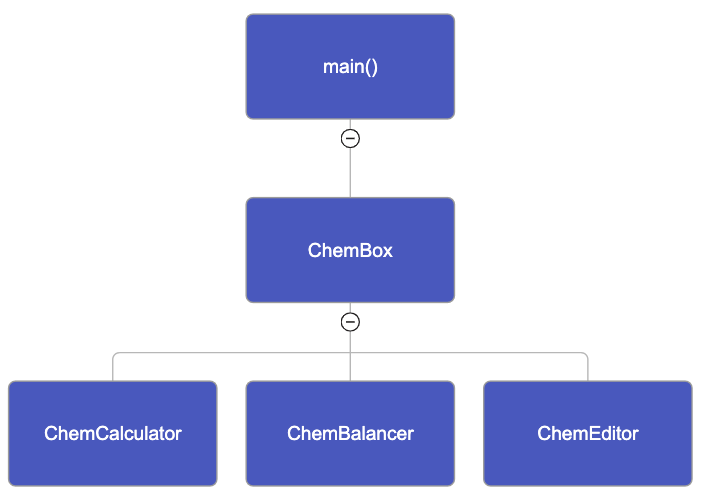
\includegraphics[scale=0.4]{base_hierarchy}
	\caption{Program Hierarchy chart}
	\label{fig:tabs_mockup}
\end{figure}

I will explain the hierarchy and program flow of the system, beginning with the ChemCalculator module.
\newpage

\subsection{Structure of the GUI}

The ChemBox class is the heart of the program, the point where all the different components are merged together to create one complete application. To give a better understanding of the system, I will explain how I composed the GUI and what each major component does. The ChemBox class contains only the constructor method, in which the layout of the graphical user interface is specified. The constructor defines the dimensions, the title and geometry of the window and then creates an instance of the TabBar class, which will act as the central widget of the program. Next, an instance of each of the three big components of the project, ChemCalculator, ChemBalancer and ChemEditor is created, and allocated to a separate tab of the tab bar (Listing 1: lines 18 - 25).

\begin{lstlisting}[language=Python, caption=Code snippet of ChemBox class No.1]
class ChemBox(QMainWindow):
    def __init__(self):
        super().__init__()

        # set window properties
        self.__left = 300
        self.__top = 300
        self.__width = 1280
        self.__height = 720
        self.__title = "ChemBox"
        self.setWindowTitle(self.__title)
        self.setGeometry(self.__left, self.__top, self.__width, self.__height)
        self.setFixedSize(self.__width, self.__height)

        self.tab_bar = TabBar()
        self.setCentralWidget(self.tab_bar)

        self.chem_calculator = ChemCalculator()
        self.tab_bar.tab1.setLayout(self.chem_calculator.main_layout)

        self.chem_balancer = ChemBalancer()
        self.tab_bar.tab2.setLayout(self.chem_balancer.balancer_layout)

        self.chem_editor = ChemEditor()
        self.tab_bar.tab3.setLayout(self.chem_editor.editor_layout)
\end{lstlisting}

\newpage
The tab bar is used as the main widget of the program at all times, as it controls the navigation between modules.
The goal was to achieve a design like the one illustrated in Figure 2, where 1, 2 and 3 in the small boxes at the top of the screen represent buttons in the tab bar for the three major modules of the ChemBox.

\begin{figure} [h]
	\centering
	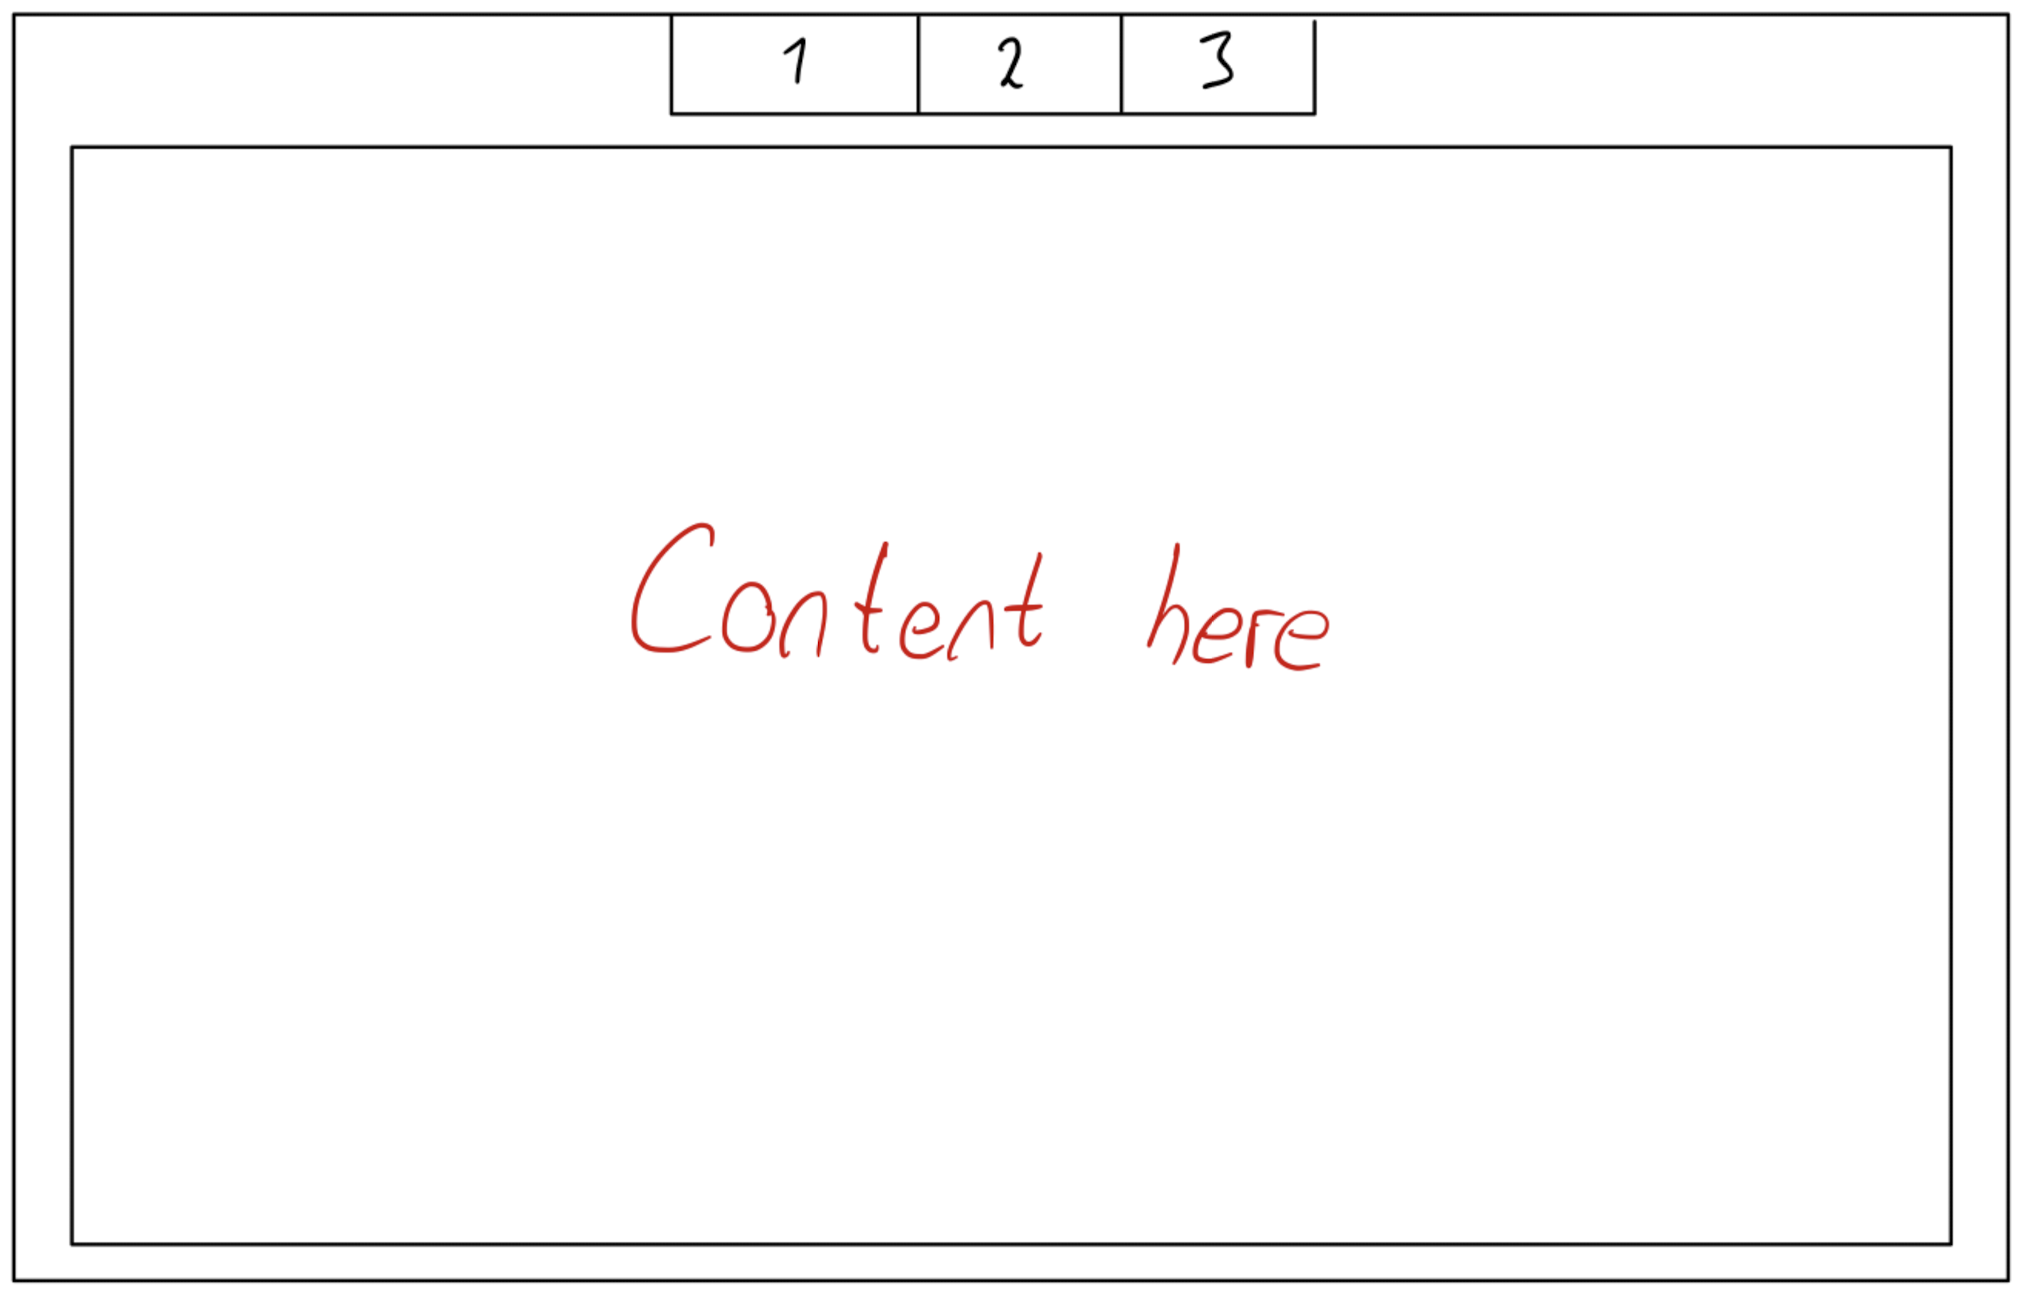
\includegraphics[scale=0.4]{tabs_mockup}
	\caption{Mockup drawing of tab bar}
	\label{fig:tabs_mockup}
\end{figure}

The ChemCalculator module is the only part of the project with a special implementation of the user interface, which needs explanation.\\

When developing the ChemCalculator module, the first issue I encountered was how I would create a layout that would work for multiple separate sub-calculators. I had three different possible systems for displaying the module. The first option was creating a sidebar, where the user can choose the exact calculator they were looking for, which is then displayed on the screen. The second option was very similar, but with an additional tab bar at the top or bottom of the screen. This solution is not very aesthetically pleasing, and could cause confusion with the actual tab bar that allows the user to switch between the three main modules. The third option was putting every calculator on the same page, each in it's own area, clearly separated from the others, and make the window scrollable. I decided against this option, as this design could have gotten very messy. Therefore, I decided to create a sidebar for the ChemCalculator. \\
As there is no built-in sidebar widget in PyQt6, I have designed my own way of creating one. I did so by using the QTabWidget, which I also used for the tab bar, but not display it. I was able to benefit from the already existing widget, for the switching between calculators, and use buttons placed on the left side of the screen as a replacement for an actual sidebar. The buttons connect to a method, which changes the the current index of the tab widget to the according number of the calculator, which updates the page that is displayed. This is illustrated in the following code snippet (Listing 2), which only includes the example on a single button, for better readability of this document.

\begin{lstlisting}[language=Python, caption=Example of ChemCalculator implementation]
class ChemCalculator(QWidget):
    def __init__(self):
        super(QWidget, self).__init__()

        self.side_bar_layout = QVBoxLayout()

        self.gibbs_calc = GibbsFreeEnergyCalculator()

        # Create buttons
        self.gibbs_free_energy_tab_button = QPushButton("Gibbs Free Energy Calculator")

        self.gibbs_free_energy_tab_button.clicked.connect(self.gibbs_free_energy_action)

        # Create tabs
        self.gibbs_free_energy_tab = QWidget()

        # Initialise gibbs free energy calculator
        self.gibbs_free_energy_tab.setLayout(self.gibbs_calc.layout)
        
        # Add buttons to sidebar layout
        self.side_bar_layout.addWidget(self.gibbs_free_energy_tab_button)

        self.side_bar_widget = QWidget()
        self.side_bar_widget.setLayout(self.side_bar_layout)

        self.page_widget = QTabWidget()

        self.page_widget.addTab(self.gibbs_free_energy_tab, "")
        
        self.page_widget.setCurrentIndex(0)
        self.page_widget.setStyleSheet('''QTabBar::tab{
        width: 0; 
        height: 0; 
        margin: 0; 
        padding: 0; 
        border: none;
        }''')

        self.main_layout = QHBoxLayout()
        self.main_layout.addWidget(self.side_bar_widget)
        self.main_layout.addWidget(self.page_widget)

        self.main_widget = QWidget()
        self.main_widget.setLayout(self.main_layout)

    # Define actions for each button
    def gibbs_free_energy_action(self):
        self.page_widget.setCurrentIndex(5)

\end{lstlisting}

\subsection{Algorithm Design for ChemCalculator}

Essential for most individual calculators in the ChemCalculator module will be an algorithm to determine which of the input options the user left blank. In general, the user interface will always consist of a number of inputs, implemented as QLineEdit's, where the blank ones are the ones that our program will calculate.\\
The algorithm will have to take a list of inputs as a parameter, and use iteration to determine the blank one.

\begin{algorithm}
\caption{Algorithm to find empty input}\label{alg:cap}
\begin{algorithmic}
\State $ input\_list \gets []$
\State $ count \gets 0$
\State $ empty\_input \gets NONE$
\For{$i \gets 0\ to\ Len(input$\_$list)$}
\If{$ input\_list[i]\ is\ empty$}
	\State $ count \gets count\ $+$\ 1$
	\State $ empty\_input \gets input\_list[i]$
\EndIf
\EndFor
\If{$ count = 1 $}
	\State $ RETURN\ count$
\EndIf
\end{algorithmic}
\end{algorithm}

\newpage

\subsection{Algorithm Design for ChemBalancer}

Figure 3 includes my initial attempt at visualising how an equation balancer could work. My first version of this module worked on a very similar system, although I struggled with finding a method of consistently balancing the equations after splitting them into their smallest possible components. 

\begin{figure} [h]
	\centering
	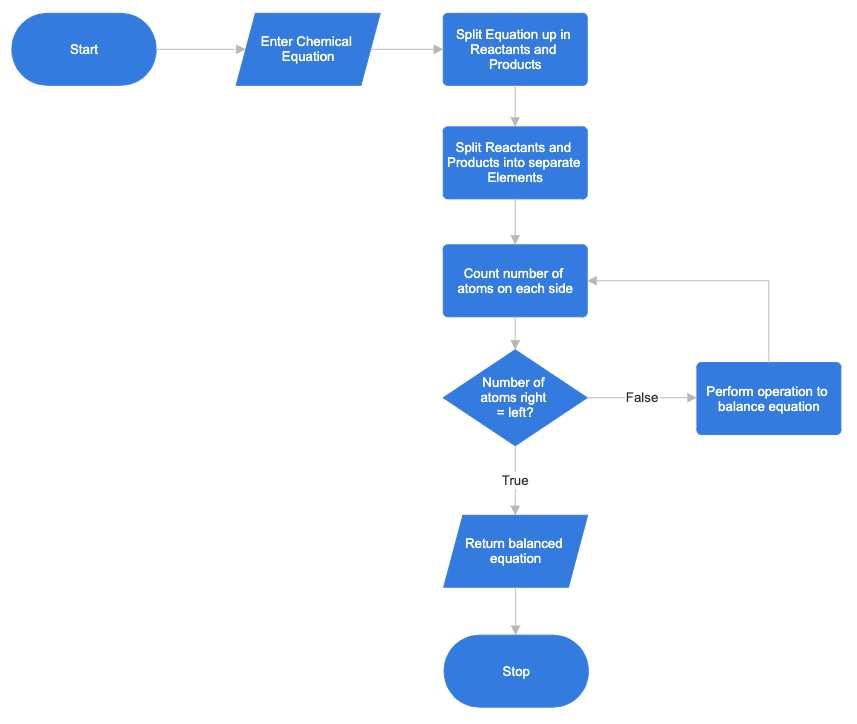
\includegraphics[scale=0.4]{balance_flow}
	\caption{Initial flowchart for balancer}
	\label{fig:balance_flow}
\end{figure}

The following code blocks contains the code of my initial, failed, attempt at the balancer.

\begin{lstlisting}[language=Python, caption=Method for splitting equation into components]
def splitEquation(self):
        self.equationSplit = self.equationInput.text().split(" = ")
        self.reactants = self.equationSplit[0]
        try:
            self.products = self.equationSplit[1]
        except IndexError:
            print("Wrong user input")
        self.reactantComponents = self.reactants.split(" + ")
        self.productComponents = self.products.split(" + ")
\end{lstlisting}

The splitEquation method uses string manipulation to extract the individual molecules of the equation and store them in separate lists for reactants and products.\\
After finding the individual molecules in the equation, the parseComponent method is called to get the elements used in the molecules, and the amount of them. This is done through if statements, as there is only a limited amount of different possibilities. The longest element symbol consists of three letters, where the first letter of every atom is always capitalised, and the following ones are not. The subscript number (number of atoms or element in a given molecule) can be found easily, as numbers within molecules always belong to the preceding element (H2O - the 2 belongs to the hydrogen). Individual elements are found by checking for capital letters. An element starts with a capital letter and ends at the next capital letter, which is where the next element starts. The same techniques were used to find brackets and complex ions in the equation.

\begin{lstlisting}[language=Python, caption=parseComponent method for finding elements]
def parseComponent(self, component, countsDict, totalDict):
        # Check for coefficient
        try:
            if component[0] in self.integers:
                try:
                    if component[0 + 1] in self.integers:
                        try:
                            if component[0 + 2] in self.integers:
                                coefficient = int(component[0: 0 + 3])
                            else:
                                coefficient = int(component[0: 0 + 2])
                        except IndexError:
                            coefficient = int(component[0: 0 + 2])
                    else:
                        coefficient = int(component[0])
                except IndexError:
                    coefficient = int(component[0])
            else:
                coefficient = 1
            for i in range(len(component)):
                try:
                    openBracket = component.find("(")
                    closedBracket = component.find(")")
                except IndexError:
                    continue
                try:
                    if component[i].isupper() and component[i - 1] != "(":
                        try:
                            if component[i + 1].islower():
                                try:
                                    if component[i + 2].islower():
                                        element = component[i:(i + 3)]
                                        if openBracket < i < closedBracket:
                                            subCoefficient = self.getSubCoefficient(component)
                                        else:
                                            subCoefficient = 1

                                        # Check for subscript
                                        try:
                                            if component[i + 3] in self.integers:
                                                try:
                                                    if component[i + 4] in self.integers:
                                                        try:
                                                            if component[i + 5] in self.integers:
                                                                subscript = int(component[(i + 3): (i + 6)])
                                                            else:
                                                                subscript = int(component[(i + 3): (i + 5)])
                                                        except IndexError:
                                                            subscript = int(component[(i + 3): (i + 5)])
                                                    else:
                                                        subscript = int(component[i + 3])
                                                except IndexError:
                                                    subscript = int(component[i + 3])
                                            else:
                                                subscript = 1
                                        except IndexError:
                                            subscript = 1
                                    else:
                                        element = component[i:(i + 2)]

                                        if openBracket < i < closedBracket:
                                            subCoefficient = self.getSubCoefficient(component)
                                        else:
                                            subCoefficient = 1

                                        # Check for subscript
                                        try:
                                            if component[i + 2] in self.integers:
                                                try:
                                                    if component[i + 3] in self.integers:
                                                        try:
                                                            if component[i + 4] in self.integers:
                                                                subscript = int(component[(i + 2): (i + 5)])
                                                        except IndexError:
                                                            subscript = int(component[(i + 2): (i + 4)])
                                                except IndexError:
                                                    subscript = int(component[i + 2])
                                            else:
                                                subscript = 1
                                        except IndexError:
                                            subscript = 1
                                except IndexError:
                                    element = component[i:(i + 2)]
                                    if openBracket < i < closedBracket:
                                        subCoefficient = self.getSubCoefficient(component)
                                    else:
                                        subCoefficient = 1
                            else:
                                element = component[i]
                                if openBracket < i < closedBracket:
                                    subCoefficient = self.getSubCoefficient(component)
                                else:
                                    subCoefficient = 1
                                try:
                                    # Check for subscript
                                    if component[i + 1] in self.integers:
                                        try:
                                            if component[i + 2] in self.integers:
                                                try:
                                                    if component[i + 3] in self.integers:
                                                        subscript = int(component[i + 1: i + 4])
                                                except IndexError:
                                                    subscript = int(component[i + 1: i + 3])
                                            else:
                                                subscript = int(component[i + 1])
                                        except IndexError:
                                            subscript = int(component[i + 1])
                                    else:
                                        subscript = 1
                                except IndexError:
                                    subscript = 1
                        except IndexError:
                            element = component[i]

                            if openBracket < i < closedBracket:
                                subCoefficient = self.getSubCoefficient(component)
                            else:
                                subCoefficient = 1

                            try:
                                # Check for subscript
                                if component[i + 1] in self.integers:
                                    try:
                                        if component[i + 2] in self.integers:
                                            try:
                                                if component[i + 3] in self.integers:
                                                    subscript = int(component[i + 1: i + 4])
                                            except IndexError:
                                                subscript = int(component[i + 1: i + 3])
                                        else:
                                            subscript = int(component[i + 1])
                                    except IndexError:
                                        subscript = int(component[i + 1])
                                else:
                                    subscript = 1
                            except IndexError:
                                subscript = 1
                        try:
                            if element in countsDict:
                                countsDict[element] = int(countsDict[element]) + subscript * coefficient * subCoefficient
                            else:
                                countsDict[element] = subscript * coefficient * subCoefficient

                            if element in totalDict:
                                totalDict[element] = int(totalDict[element]) + subscript * coefficient * subCoefficient
                            else:
                                totalDict[element] = subscript * coefficient * subCoefficient
                        except UnboundLocalError:
                            continue

                    # Check for brackets / complex ion in equation
                    elif component[i] == "(":
                        try:
                            if component[i + 2] == ")":
                                element = component[i + 1]
                                try:
                                    if component[i + 3] in self.integers:
                                        try:
                                            if component[i + 4] in self.integers:
                                                try:
                                                    if component[i + 5] in self.integers:
                                                        subscript = int(component[(i + 3): (i + 6)])
                                                    else:
                                                        subscript = int(component[(i + 3): (i + 5)])
                                                except IndexError:
                                                    subscript = int(component[(i + 3): (i + 5)])
                                            else:
                                                subscript = int(component[(i + 3): (i + 4)])
                                        except IndexError:
                                            subscript = int(component[i + 3])
                                    else:
                                        subscript = 1
                                except IndexError:
                                    subscript = 1
                            elif component[i + 1].isupper():
                                if component[i + 2].islower():
                                    try:
                                        if component[i + 3].islower():
                                            element = component[(i + 1): (i + 4)]

                                            # Check for subscript within brackets
                                            try:
                                                if component[i + 4] in self.integers:
                                                    try:
                                                        if component[i + 5] in self.integers:
                                                            try:
                                                                if component[i + 6] in self.integers:
                                                                    subscript = int(component[(i + 4): (i + 7)])
                                                                else:
                                                                    subscript = int(component[(i + 4): (i + 6)])
                                                            except IndexError:
                                                                subscript = int(component[(i + 4): (i + 6)])
                                                        else:
                                                            subscript = int(component[i + 4])
                                                    except IndexError:
                                                        subscript = int(component[i + 4])
                                                else:
                                                    subscript = 1
                                            except IndexError:
                                                subscript = 1

                                            # Find subscript coefficient of complex ion
                                            subCoefficient = self.getSubCoefficient(component)
                                        else:
                                            element = component[(i + 1): (i + 3)]

                                            # Check for subscript within brackets
                                            try:
                                                if component[i + 3] in self.integers:
                                                    try:
                                                        if component[i + 4] in self.integers:
                                                            try:
                                                                if component[i + 5] in self.integers:
                                                                    subscript = int(component[(i + 3): (i + 6)])
                                                                else:
                                                                    subscript = int(component[(i + 3): (i + 5)])
                                                            except IndexError:
                                                                subscript = int(component[(i + 3): (i + 5)])
                                                    except IndexError:
                                                        subscript = int(component[i + 3])
                                                else:
                                                    subscript = 1
                                            except IndexError:
                                                subscript = 1

                                            # Find subscript coefficient of complex ion
                                            subCoefficient = self.getSubCoefficient(component)
                                    except IndexError:
                                        element = component[(i + 1): (i + 3)]

                                        # Check for subscript within brackets
                                        try:
                                            if component[i + 3] in self.integers:
                                                try:
                                                    if component[i + 4] in self.integers:
                                                        try:
                                                            if component[i + 5] in self.integers:
                                                                subscript = int(component[(i + 3): (i + 6)])
                                                            else:
                                                                subscript = int(component[(i + 3): (i + 5)])
                                                        except IndexError:
                                                            subscript = int(component[(i + 3): (i + 5)])
                                                except IndexError:
                                                    subscript = int(component[i + 3])
                                            else:
                                                subscript = 1
                                        except IndexError:
                                            subscript = 1

                                        # Find subscript coefficient of complex ion
                                        subCoefficient = self.getSubCoefficient(component)
                                else:
                                    element = component[i + 1]

                                    # Check for subscript within brackets
                                    try:
                                        if component[i + 2] in self.integers:
                                            try:
                                                if component[i + 3] in self.integers:
                                                    try:
                                                        if component[i + 4] in self.integers:
                                                            subscript = int(component[(i + 2): (i + 5)])
                                                        else:
                                                            subscript = int(component[(i + 2): (i + 4)])
                                                    except IndexError:
                                                        subscript = int(component[(i + 2): (i + 4)])
                                            except IndexError:
                                                subscript = int(component[i + 2])
                                        else:
                                            subscript = 1
                                    except IndexError:
                                        subscript = 1

                                    # Find subscript coefficient of complex ion
                                    subCoefficient = self.getSubCoefficient(component)
                        except IndexError:
                            print("wrong user input ")
                        try:
                            if element in countsDict:
                                countsDict[element] += subscript * subCoefficient * coefficient
                            else:
                                countsDict[element] = subscript * subCoefficient * coefficient
                            if element in totalDict:
                                totalDict[element] += subscript * subCoefficient * coefficient
                            else:
                                totalDict[element] = subscript * subCoefficient * coefficient
                        except UnboundLocalError:
                            continue
                    else:
                        continue
                except IndexError:
                	continue
        except IndexError:
            None
\end{lstlisting}

Although this code is overly complicated, it worked most of the times for basic or intermediate level equations.\\
The main problem this version of the balancer ran into, was the actual balancing of the equations. The version uses a loop to attempt balancing, where copies of the left and right hand side components are created together with dictionaries to track the total count of elements. Each component then gets a randomly generated coefficient between 1 and 10, and the loop continues until the count on the left side equals the count on the right side. Once a balanced equation is found, the coefficients are normalised to their smallest integer values using the greatest common divisor (GCD) The balanced equation is then put back together and returned to the user.\\

\begin{lstlisting}[language=Python, caption=balance method]
def balance(self):
        if self.balanced:
            equation = str()
            for dictionary in self.left:
                compound = str()
                for element in dictionary:
                    compound += element
                    if dictionary[element] > 1:
                        compound += str(dictionary[element])
                equation += compound
                equation += " + "
            equation = equation[:len(equation) - 3] + " = "
            for dictionary in self.right:
                compound = str()
                for element in dictionary:
                    compound += element
                    if dictionary[element] > 1:
                        compound += str(dictionary[element])
                    else:
                        pass
                equation += compound
                equation += " + "
            equation = equation[:len(equation) - 2]
        else:
            while not self.balanced:
                tempLeft = list()
                tempRight = list()
                totalLeft = dict()
                totalRight = dict()

                for item in self.left:
                    newDict = dict()
                    for key in item:
                        newDict[key] = item[key]
                    tempLeft.append(newDict)

                for item in self.right:
                    newDict = dict()
                    for key in item:
                        newDict[key] = item[key]
                    tempRight.append(newDict)

                leftCoefficients = [randint(1, 10) for _ in range(len(tempLeft))]
                rightCoefficients = [randint(1, 10) for _ in range(len(tempRight))]

                for index in range(0, len(leftCoefficients)):
                    for key in tempLeft[index]:
                        tempLeft[index][key] *= leftCoefficients[index]
                        if key not in totalLeft:
                            totalLeft[key] = tempLeft[index][key]
                        else:
                            totalLeft[key] += tempLeft[index][key]

                for index in range(0, len(rightCoefficients)):
                    for key in tempRight[index]:
                        tempRight[index][key] *= rightCoefficients[index]
                        if key not in totalRight:
                            totalRight[key] = tempRight[index][key]
                        else:
                            totalRight[key] += tempRight[index][key]

                self.balanced = True
                for key in totalLeft:
                    if totalLeft[key] != totalRight[key]:
                        self.balanced = False
                    else:
                        continue

            bigTup = tuple(leftCoefficients + rightCoefficients)
            leftCoefficients = list(map(lambda x: int(x / reduce(gcd, bigTup)), leftCoefficients))
            rightCoefficients = list(map(lambda x: int(x / reduce(gcd, bigTup)), rightCoefficients))

            balancedEquation = str()
            for index in range(0, len(self.left)):
                if leftCoefficients[index] != 1:
                    compound = str(leftCoefficients[index])
                else:
                    compound = str()
                for key in self.left[index]:
                    compound += key
                    if self.left[index][key] != 1:
                        compound += str(self.left[index][key])
                balancedEquation += compound
                balancedEquation += " + "
            balancedEquation = balancedEquation[:len(balancedEquation) - 3] + " = "
            for index in range(0, len(self.right)):
                if rightCoefficients[index] != 1:
                    compound = str(rightCoefficients[index])
                else:
                    compound = str()
                for key in self.right[index]:
                    compound += key
                    if self.right[index][key] != 1:
                        compound += str(self.right[index][key])
                balancedEquation += compound
                balancedEquation += " + "
            balancedEquation = balancedEquation[:len(balancedEquation) - 2]
            return self.balancedLabel.setText(f"{balancedEquation}")
\end{lstlisting}

\newpage

This version had a few obvious limitations, it relied on randomly generated coefficients, which is not a very reliable system of finding the correct coefficients. Although the random generation usually provides coefficients, it  may not always produce the most optimal or smallest possible coefficients. The normalisation step using the greatest common divisor ensures that the coefficients are integer multiples of each other, but it does not guarantee the smallest 	possible coefficients. If a balanced equation cannot be found with the randomly generated coefficients, there is also a possibility of infinite looping.

\begin{figure} [h]
	\centering
	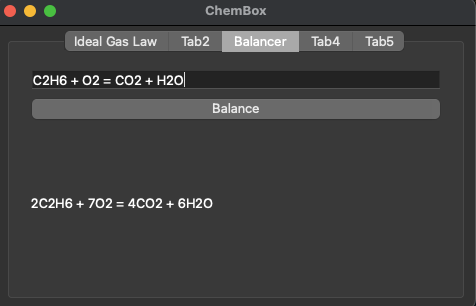
\includegraphics[scale=0.5]{initial_balance_test}
	\caption{Initial balancer test}
	\label{fig:initial_balance_test}
\end{figure}

The test in Figure 4 shows, that the system works (at least for simple equations). Just the simple addition of two carbon atoms and four hydrogen atoms to get the equation $ C2H6 + O2 = CO2 + H2O$ is already too much for the system, as this will end in an infinite loop. This loop can be prevented by increasing the range of possibilities for the randomly generated integers (for example from between 1 and 10 to between 1 and 100) but this means there is always a limit to what is possible for the balancer. Figure 5 shows the state of the program after trying to balance the equation with the original range of one to 10. The program in the figure is in the state of an infinite loop.

\begin{figure} [h]
	\centering
	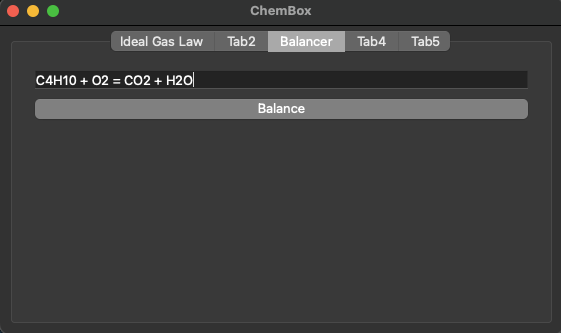
\includegraphics[scale=0.5]{initial_balance_test2}
	\caption{Initial balancer test No. 2}
	\label{fig:initial_balance_test2}
\end{figure}

\newpage

Whilst researching for better ways to implement a chemical equation balancer in python, I came across regular expressions, which around that same time, we also covered in out A-Level Computer Science lessons. Knowing about regular expressions helped me significantly improve the effectiveness of my balancer, when it comes to extracting individual elements and their amount from the equation. In my search for the best possible way to do so, I wrote a number of algorithms, which extend each other perfectly, to finish the job together.\\
This algorithm (Algorithm 2) takes the full equation as a parameter from the user input and removes any whites paces from it. It then splits it up into separate reactants and products, and lastly, it extracts the individual reagents within the reactants and products.
\begin{algorithm}
\caption{Algorithm to split equation}\label{alg:cap}
\begin{algorithmic}
\Function{$ split\_equation$}{$ $}
\State $ stripped\_equation \gets USERINPUT$
\State $ stripped\_equation \gets stripped\_equation.STRIP(" ")$
\State $ equation\_split \gets stripped\_equation.SPLIT("=")$
\State $ reactants \gets equation\_split[0].SPLIT("+")$
\State $ products \gets equation\_split[1].SPLIT("+")$
\EndFunction
\end{algorithmic}
\end{algorithm}

This second algorithm(Algorithm 3), which I designed for the task mentioned above, uses regular expressions, to identify separate reagents within a chemical compound by identifying brackets. The goal is to split up compounds like $ CuNO3)2$ into $ ["Cu",\ "(NO3)2"]$, where $Cu$ and $(NO3)2$ are two separate entries in the list. The method then iterates over each reagent, and checks if it starts with an opening bracket. If it does, this indicates, that there is a chemical compound enclosed in the brackets. It extracts the inner compound and the subscript ($ (OH)2$ indicates that the $(OH)$ group exists twice), and then passes these two variables as parameters to the "find\_elements" method, along with the "index" and "side" parameters.

\begin{algorithm}
\footnotesize
\caption{Algorithm to find reagents}\label{alg:cap}
\begin{algorithmic}
\Function{$find\_reagents$}{$compound,\ index,\ side$}
\State $ reagents \gets SPLIT\ compound\ INTO\ reagents\ USING\ REGEX\ PATTERN$
\For{$ reagent\ IN\ reagents$}
\If{$ reagent\ BEGINS\ WITH\ "("$}
	\State $ inner\_compound \gets SUBSTRING(1,\ LEN(reagent))$
	\State $ bracket\_subscript \gets SPLIT\ reagent\ BY\ ")"\ AND\ GET\ SECOND\ PART$
	\If{$ bracket\_subscript\ EXISTS$}
		\State $ bracket\_subscript \gets INT(bracket\_subscript)$
	\Else
		\State $ bracket\_subscript \gets 1$
	\EndIf
	\State $ find\_elements(inner\_compound,\ index,\ bracket\_subscript,\ side)$
\Else
	\State $ bracket\_subscript \gets 1$
	\State $ find\_elements(reagent,\ index,\ bracket\_subscript,\ side)$
\EndIf
\EndFor
\EndFunction
\end{algorithmic}
\end{algorithm}

The next algorithm (Algorithm 4) uses a regular expression to obtain the elements and associated subscript values. Each extracted element is then stored together with the correlated subscript value as a tuple, inside a list (For example: $Cr2O7$ $\rightarrow$ $[("Cr",\ "2"),\ ("O",\ "7")]$). The algorithm then iterates through each tuple (elements, subscript) in the element\_counts list.
With every iteration, a different subroutine named add\_to\_matrix is called, passing the current element, index, the product of the bracket\_subscript and subscript, and the side argument.

\newpage

\begin{algorithm}
\footnotesize
\caption{Algorithm to find elements}\label{alg:cap}
\begin{algorithmic}
\Function{$find\_reagents$}{$reagent,\ index,\ bracket\_subscript,\ side$}
\State $ element\_counts \gets SPLIT\ reagent\ INTO\ element\_counts\ USING\ REGEX\ PATTERN$
\For{$ element,\ subscript\ IN\ element\_counts$}
\If{$ subscript\ DOES\ NOT\ EXIST$}
	\State $ subscript \gets 1$
\Else
	\State $ subscript \gets INT(subscript)$
\EndIf
\State $ add\_to\_matrix(element,\ index,\ bracket\_subscript * subscript,\ side)$
\EndFor
\EndFunction
\end{algorithmic}
\end{algorithm}

While I was conducting my research, I found a neat solution to balancing equations, matrix operations. As we had only covered the rudimentary principles of matrix operations, I chose to use the article I had found on the internet to get a better understanding of the topic. After getting a grasp of the concept, and after trying out the code in the article, I had found a different way to tackle my problem. I decided not to reinvent the wheel, but to take the already existing algorithm and improve it, so it could be used for practically any tractable equation there is.\\
To address the problem, I decided to record a number of issues and possible improvements for the existing algorithm.

\begin{enumerate}
\item The first issue I had with the algorithm was, that it asked for separate inputs of reactants and products. Luckily, I had already solved this problem with the algorithms illustrated earlier.
\item Another issue the original algorithm had was the lack of structure and modularity. By organising the code in a class based structure, I ensured good readability for the code, as well as making it easier to maintain.
\item The original version had poor input validation and error handling. One common error I got with the early implementation of the algorithm was what I call a nullspace error. The nullspace is a linear subspace that contains a set of vectors that transform to the zero$^{th}$ vector under a given linear transformation: multiplication with the matrix A, represented as $ Ax = 0$. In the context of chemical equations, the nullspace contains the coefficients, that balance the equation.\\
Entering the unbalanced equation $ K4[Fe(SCN)6] + K2Cr2O7 + H2SO4$\\ $ = Fe2(SO4)3 + Cr2(SO4)3 + CO2 + H2O + K2SO4 + KNO3$ resulted in a "nullspace error" (Figure 6). 

\newpage

\begin{figure} [h]
	\centering
	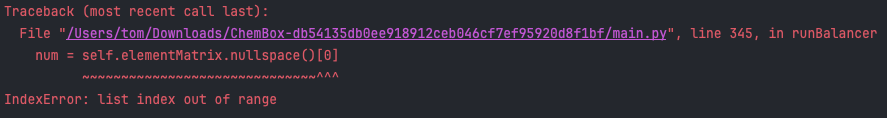
\includegraphics[scale=0.4]{nullspace_error}
	\caption{Nullspace error}
	\label{fig:nullspace_error}
\end{figure}

I managed to neutralise this error by having a more accurate and efficient method of separating out molecules, elements, etc. as shown in Algorithm 3 and Algorithm 4, before passing them on to the method that adds the items to the matrix.\\
I also made sure to use pythons built in exception handling to catch any expected and unexpected errors or exceptions.
\end{enumerate}

Using the current working system, inputting the chemical equation mentioned before results in a perfectly balanced equation (Figure 7).

\begin{figure} [h]
	\centering
	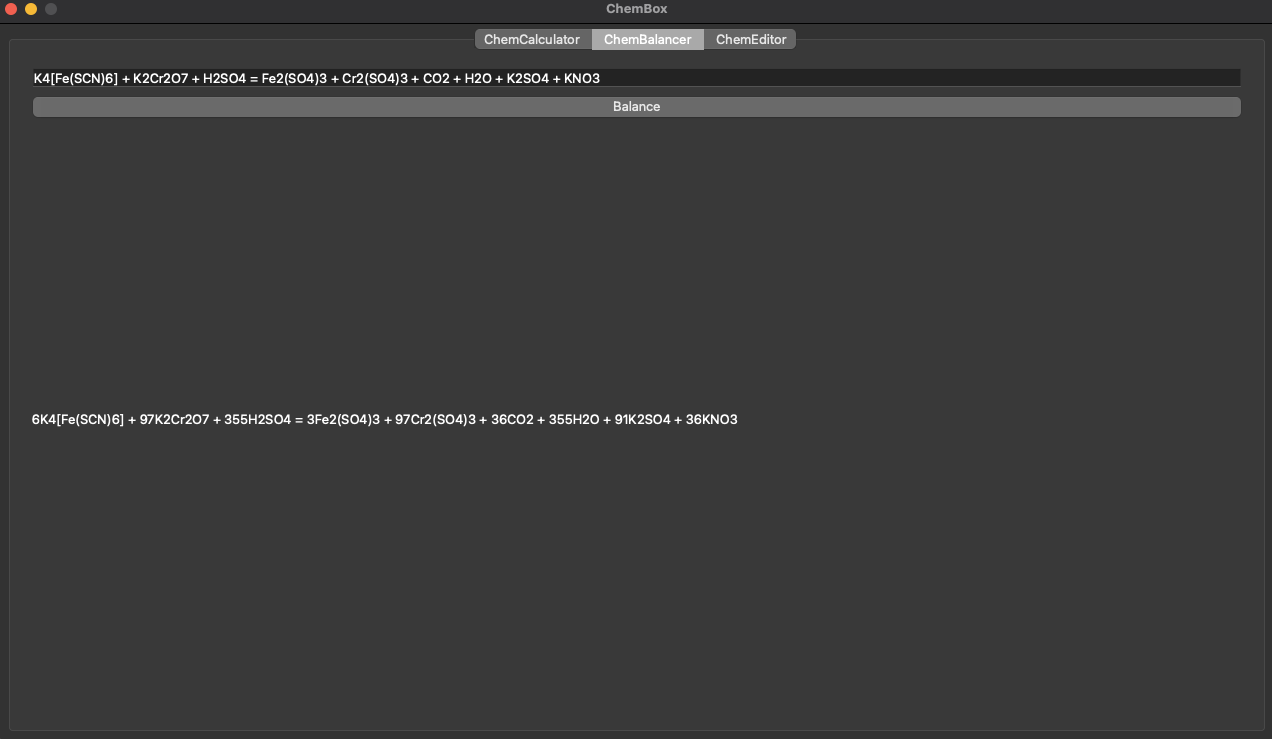
\includegraphics[scale=0.3]{working_balancer}
	\caption{Balanced equation}
	\label{fig:working_balancer}
\end{figure}

\newpage

\section{Testing}

\section{Evaluation}
\newpage

\end{document}
